\section{Random Variables}
A \textbf{random variable}, $\tilde{x}$, is a mathematical representation of a value and its associated uncertainty. Usually, we are interested not just in the behaviour of a certain value of a variable or parameter, but also in how it behaves when it is uncertain. A \textit{sample} of such random variable can take several values according some \textbf{distribution law}. So we are specially interested in how this distribution law \textit{reshapes} when passing through different physical processes and/or computation steps. The \textbf{probability density function}, also known as PDF, or just \textit{density}, is a function 
\begin{equation}
F_{\tilde{x}}(x):\mathbb{R}\rightarrow \mathbb{R} 
\end{equation}
that expresses which values in the domain of the variable $x$ are more likely, according to the random variable $\tilde{x}$. However, since this function is a density, the actual value expressing a probability is the integral between an interval:
\begin{equation}
p(a<\tilde{x}<b) = \int^b_a F_{\tilde{x}}(x) dx 
\end{equation}

A \textbf{random vector}, $\tilde{\mathbf{x}}$, is an array of random variables, stacked forming a column vector: 
\begin{equation}
\tilde{\mathbf{x}} =
\left[
\begin{array}{c}
 \tilde{x}_1\\
 \tilde{x}_2\\
 \vdots \\
 \tilde{x}_n\\
\end{array}
\right].
\end{equation}
In such case, the probability density function is defined as: 
\begin{equation}
F_{\tilde{\mathbf{x}}}(\mathbf{x}):\mathbb{R}^n\rightarrow \mathbb{R} 
\end{equation}
and the probability in a given interval,~$I$, is computed as:
\begin{equation}
p(\tilde{\mathbf{x}}\in I) = 
p(a_n<\tilde{x}_1<b_n,\dots,a_n<\tilde{x}_n<b_n) = 
\int^{b_1}_{a_1} \dots \int^{b_n}_{a_n} F_{\tilde{\mathbf{x}}}(\mathbf{x}) dx_n \dots dx_1 
\end{equation}

\subsection{Moments}
A way to parameterize a distribution law is through its \textit{moments}, a set of parameters that can fully describe the distribution in some cases, or just approximate it in others. The most known moments are the mean, $\mu$, which is the fisrt order moment, and the variance, $\sigma^2$, which is the second order moment. %Third and fourth order moments are called skewness and kurtoise.  

From a set of $n$ samples $\{x_1\dots x_n\}$, $x_i \in\mathbb{R}$, the mean and variance can be estimated as:
\begin{equation}
 \mu_x = \frac{1}{n}\sum^n_{i=1} x_i;\ \ \ \sigma^2_x = \frac{1}{n-1}\sum^n_{i=1} (x_i-\mu_x)^2;
\end{equation}

In the multivariate case the mean becomes a vector, so it can be estimated as:
\begin{equation}
 \boldsymbol\mu_x = \frac{1}{n}\sum^n_{i=1} \mathbf{x}_i;
\end{equation}
and the second order moment can be \textit{cross}computed, so a \textit{covariance} matrix is used to describe this second order stathistics. This matrix is squared, and from a set of samples can be estimated as: 
\begin{equation}
 \mathbf{C}_x = 
 \left[
 \begin{array}{ccccccc}
  c11 &  & & & c1j &  & c1n \\
  \vdots & & & \ddots & \vdots & & \vdots \\
  ci1 &  & cii & & & & cin \\
  \vdots & & & \vdots & \ddots & & \vdots \\
  \vdots & & & & cij & & \vdots \\
  \vdots & & & \vdots & \ddots & & \vdots \\
  cn1 &  & & cnj & & & cnn \\
 \end{array}
 \right]
\end{equation}

%comments about main directions represented in the covariance matrix. 
%example drawing an ellipses from a covariance matrix
%example drawing a bbox from a covariance matrix
%example PCA


\subsection{Uniform distribution}
A random variable or vector is called uniform when the density is constant over a bounded interval, meaning that the variable is equally distributed within this interval. That implies also that the variable can take, with equal probability, values within this interval. 

Uniform random variables can be described with just two parameters: $x_{min}, x_{max}$. The mean and the variance values of an unfiorm random variable are:
\begin{equation}
 \mu_{\tilde{x}} = \frac{x_{min}+x_{max}}{2}; \ \ 
 %\sigma^2_{\tilde{x}} = //TODO
\end{equation}

% \begin{table}[h]
% \caption{Example of C++/std code for uniform random generator}
% \begin{tabular}
% [l]{|l|}
% \hline
% \rowcolor{Gray} \ttfamily \#include xx \\
% \rowcolor{Gray} \ttfamily void main() \\
% \rowcolor{Gray} \ttfamily \{ \\
% \rowcolor{Gray} \ttfamily \hspace{1cm} //TODO; 
% \rowcolor{Gray} \ttfamily \} \\
% \hline
% \end{tabular}
% \label{tab:random}
% \end{table}

\subsection{Gaussian distribution}
A random variable is called Gaussian or Normal, when its density is fully described with two parameters, $\mu_{\tilde{x}}$ (mean) and $\sigma^2_{\tilde{x}}$ (standard deviation), and the following expression:
\begin{equation}
 F_{\tilde{x}}(x) = \frac{1}{2\pi}e^{-(\frac{x-\mu_{\tilde{x}}}{\sigma_{\tilde{x}}})^2}
\end{equation}
Gaussian variables are also written as $\mathcal{N}(\mu,\sigma)$, which is a widely used notation stressing the dependency with just two parameters. Given $\tilde{x}=\mathcal{N}(\mu_x,\sigma_x)$ and $\tilde{y}=\mathcal{N}(\mu_y,\sigma_y)$, the following properties fulfill:
\begin{itemize}
 \item $\tilde{z}=a\tilde{x} \ \ \rightarrow \tilde{z}=\mathcal{N}(a\mu_x,a\sigma_x)$
 \item $\tilde{z}=\tilde{x}+\tilde{y} \ \ \rightarrow \tilde{z}=\mathcal{N}(\mu_x+\mu_y,\sqrt{\sigma^2_x+\sigma^2_y})$
\end{itemize}
The two properties listed above are of major importance since they imply that we know how Gaussian variables behave when they pass through linear systems. 

%example code for normal random generator and then computation of mean and variance

\subsection{Multivariate Gaussian distribution}
In case of $n$-dimensional Gaussian variables, the mean is $\boldsymbol{\mu} \in \mathbb{R}^n$, and the covariance is represented as a squared matrix, $\mathbf{C}\in\mathbb{R}^{n\times n}$. The generalized formula is the following: 
\begin{equation}
 F_{\tilde{x}}(\mathbf{x}) = \frac{1}{\sqrt{\vert \mathbf{C}\vert}(2\pi)^n}
			    e^{-\frac{1}{2}(\mathbf{x}-\boldsymbol\mu)^T\mathbf{C}^{-1}(\mathbf{x}-\boldsymbol\mu)}
\end{equation}

\begin{figure}[bth!]
  \begin{center}
    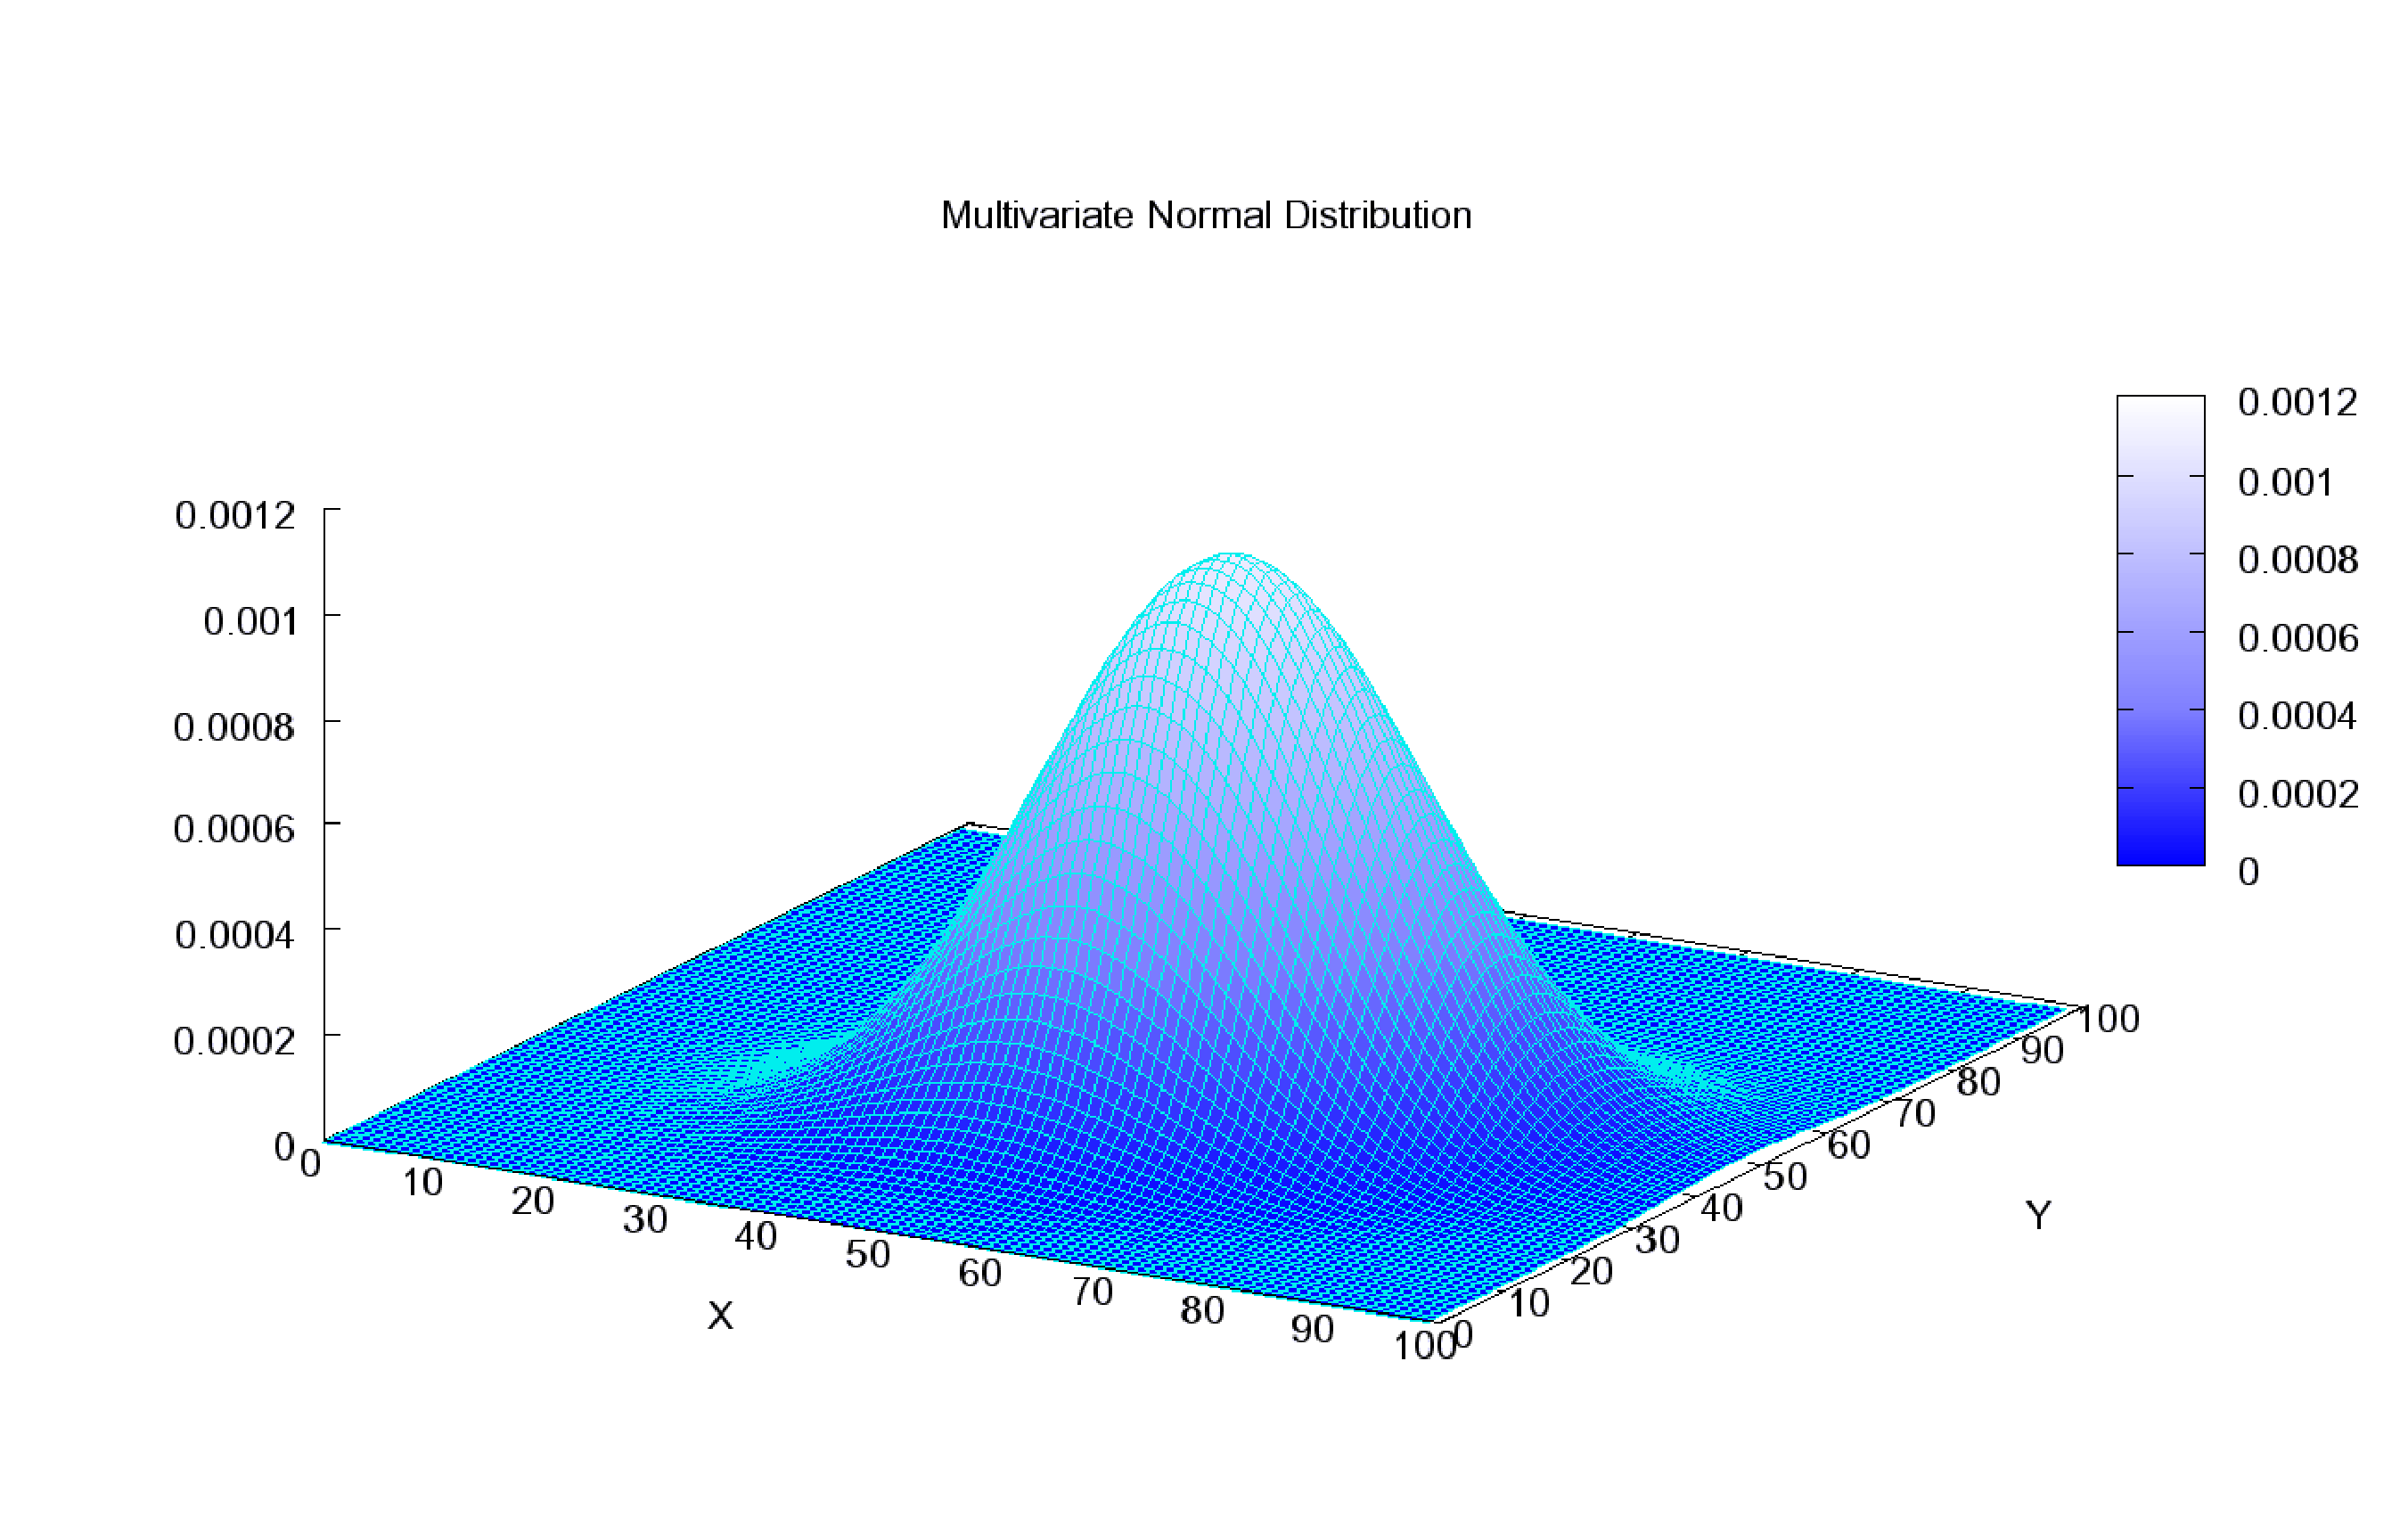
\includegraphics[width=1.0\columnwidth]{figures/mv_gaussian.eps}
    \caption{Bivariate Gaussian function}
    \label{fig:trigonometry}
  \end{center}
\end{figure}

The main operations are,



\subsection{Gaussian Uncertainty Propagation}
How uncertainty is propagated through different physical or computing processes is a major topic in robotics, specially in perception, but also in precise actuation. Specifically, we are interested in know how a density function reshapes due to some computation, view point change, ...

In previous subsections we've seen that Gaussian random variables and vectors have the great property that it is easy (conceptually, but computationally also) to compute their parameters once they pass through linear operations (product by scalar and sum). We've also seen in section~\ref{sec:Linearization} that non-linear functions can be linearized, by assuming a linearization error. Therefore, linearization and Gaussian uncertainty propagation are two operations very common in many robotics algorithms. 

//procedure: TODO: vector function, Jacobian, $APA^T$


